% LaTeX Figure Portfolio — Demonstration Document
% Shows: theorem/algorithm environments, BibTeX, and TikZ/PGFPlots figures
% Compile:  pdflatex portfolio && bibtex portfolio && pdflatex portfolio && pdflatex portfolio

\documentclass[11pt,a4paper]{article}

% ---- Math & theorems ----
\usepackage{amsmath,amssymb,amsthm}
\newtheorem{theorem}{Theorem}[section]
\newtheorem{lemma}[theorem]{Lemma}
\newtheorem{proposition}[theorem]{Proposition}
\newtheorem{corollary}[theorem]{Corollary}
\theoremstyle{definition}
\newtheorem{definition}[theorem]{Definition}
\newtheorem{example}[theorem]{Example}
\theoremstyle{remark}
\newtheorem*{remark}{Remark}

% ---- Graphics ----
\usepackage{tikz}
\usepackage{pgfplots}
\pgfplotsset{compat=1.18}
\usetikzlibrary{arrows.meta,calc,positioning,decorations.pathreplacing,fit,shapes.geometric}

% ---- Algorithms ----
\usepackage{algorithm}
\usepackage{algpseudocode}

% ---- Typography & layout ----
\usepackage[margin=2.5cm]{geometry}
\usepackage{hyperref}
\hypersetup{colorlinks=true,linkcolor=blue!60!black,citecolor=green!50!black}

% ---- Bibliography (traditional bibtex) ----
\bibliographystyle{plain}

% ---- Custom colors for figures ----
\definecolor{accent}{RGB}{26,82,118}
\definecolor{accent2}{RGB}{192,57,43}
\definecolor{accent3}{RGB}{39,174,96}

\title{\LaTeX{} Figure Portfolio\\[4pt]
\large A demonstration of theorem environments, algorithm typesetting,\\
BibTeX, and TikZ/PGFPlots figures}
\author{[YOUR NAME]}
\date{\today}

\begin{document}
\maketitle
\tableofcontents
\newpage

% =====================================================================
\section{Theorem environments and cross-references}
% =====================================================================

This section demonstrates the standard \texttt{amsthm} theorem environments
with automatic numbering and cross-referencing.

\begin{definition}[Convex function]
\label{def:convex}
A function $f : \mathbb{R}^n \to \mathbb{R}$ is \emph{convex} if for all
$x, y \in \mathbb{R}^n$ and $\theta \in [0,1]$:
\begin{equation}
\label{eq:convex_def}
f(\theta x + (1-\theta) y) \le \theta f(x) + (1-\theta) f(y).
\end{equation}
\end{definition}

\begin{theorem}[First-order optimality]
\label{thm:first_order}
Let $f : \mathbb{R}^n \to \mathbb{R}$ be convex and differentiable. Then
$x^*$ is a global minimizer of $f$ if and only if $\nabla f(x^*) = 0$.
\end{theorem}

\begin{proof}
If $\nabla f(x^*) = 0$, then by convexity (Definition~\ref{def:convex}),
$f(y) \ge f(x^*) + \langle \nabla f(x^*),\, y - x^* \rangle = f(x^*)$
for all $y$, so $x^*$ is a global minimizer. The converse is immediate
since $f$ is differentiable.
\end{proof}

\begin{lemma}[Coercivity of the augmented Lagrangian]
\label{lem:coercive}
Let $L_\rho(x, y) = f(x) + \langle y, Ax - b \rangle + \frac{\rho}{2}\|Ax - b\|^2$.
If $f$ is coercive and $A$ has full column rank, then $L_\rho(\cdot, y)$
is coercive for every $y$ and $\rho > 0$.
\end{lemma}

By Theorem~\ref{thm:first_order} and Lemma~\ref{lem:coercive}, the
$x$-update in ADMM has a unique minimizer under mild conditions
(see Algorithm~\ref{alg:admm} below).

% =====================================================================
\section{Algorithm typesetting}
% =====================================================================

\begin{algorithm}[t]
\caption{Alternating Direction Method of Multipliers (ADMM)}
\label{alg:admm}
\begin{algorithmic}[1]
\Require problem data $A, b$, penalty $\rho > 0$, tolerance $\varepsilon$
\Ensure approximate solution $x^*$
\State Initialize $x^0, z^0, u^0$
\For{$k = 0, 1, 2, \dots$}
  \State $x^{k+1} \gets \arg\min_x\ f(x) + \frac{\rho}{2}\|x - z^k + u^k\|^2$
  \State $z^{k+1} \gets \arg\min_z\ g(z) + \frac{\rho}{2}\|x^{k+1} - z + u^k\|^2$
  \State $u^{k+1} \gets u^k + x^{k+1} - z^{k+1}$
  \If{$\|x^{k+1} - z^{k+1}\| \le \varepsilon$ \textbf{and} $\|z^{k+1} - z^k\| \le \varepsilon$}
    \State \Return $x^{k+1}$
  \EndIf
\EndFor
\end{algorithmic}
\end{algorithm}

% =====================================================================
\section{TikZ figures}
% =====================================================================

% ---- Figure 1: ADMM convergence (PGFPlots) ----
\begin{figure}[t]
\centering
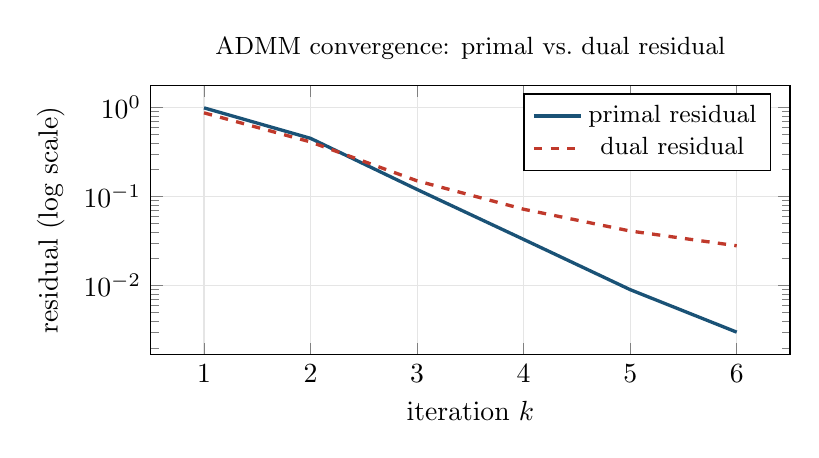
\begin{tikzpicture}
\begin{axis}[
  width=0.8\textwidth, height=5cm,
  xlabel={iteration $k$}, ylabel={residual (log scale)},
  ymode=log, grid=major, grid style={gray!20},
  legend pos=north east, legend style={font=\small},
  title={\small ADMM convergence: primal vs.\ dual residual}
]
\addplot[accent, very thick, mark=none] coordinates {
  (1,0.99)(2,0.45)(3,0.12)(4,0.033)(5,0.009)(6,0.003)
};
\addlegendentry{primal residual}
\addplot[accent2, very thick, dashed, mark=none] coordinates {
  (1,0.87)(2,0.41)(3,0.15)(4,0.072)(5,0.041)(6,0.028)
};
\addlegendentry{dual residual}
\end{axis}
\end{tikzpicture}
\caption{ADMM primal and dual residuals for the LASSO problem.
Both residuals decrease geometrically in early iterations.}
\label{fig:admm_conv}
\end{figure}

% ---- Figure 2: Function plots (PGFPlots) ----
\begin{figure}[t]
\centering
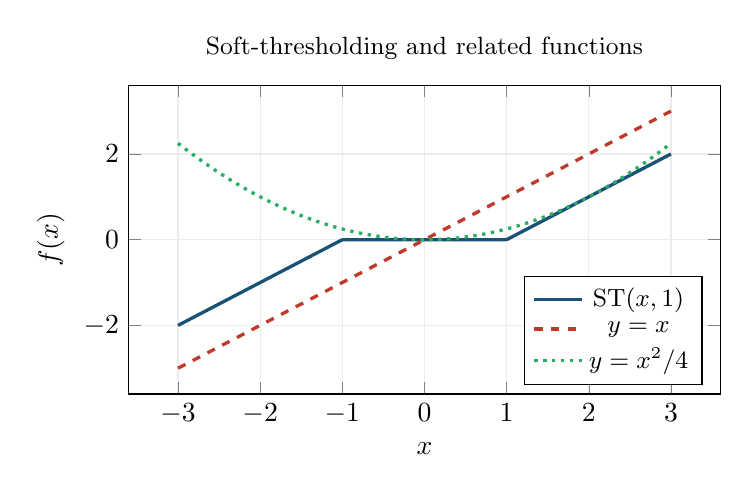
\begin{tikzpicture}
\begin{axis}[
  width=0.75\textwidth, height=5.5cm,
  xlabel={$x$}, ylabel={$f(x)$},
  grid=major, grid style={gray!15},
  legend pos=south east, legend style={font=\small},
  title={\small Soft-thresholding and related functions}
]
\addplot[accent, very thick, domain=-3:3, samples=200] {max(abs(x)-1, 0)*sign(x)};
\addlegendentry{$\mathrm{ST}(x, 1)$}
\addplot[accent2, very thick, dashed, domain=-3:3, samples=200] {x};
\addlegendentry{$y = x$}
\addplot[accent3, very thick, dotted, domain=-3:3, samples=200] {x^2/4};
\addlegendentry{$y = x^2/4$}
\end{axis}
\end{tikzpicture}
\caption{The soft-thresholding operator $\mathrm{ST}(x,\tau) = \mathrm{sign}(x)\max(|x|-\tau,0)$
compared with the identity and quadratic.}
\label{fig:soft_threshold}
\end{figure}

% ---- Figure 3: Algorithm flowchart (TikZ) ----
\begin{figure}[t]
\centering
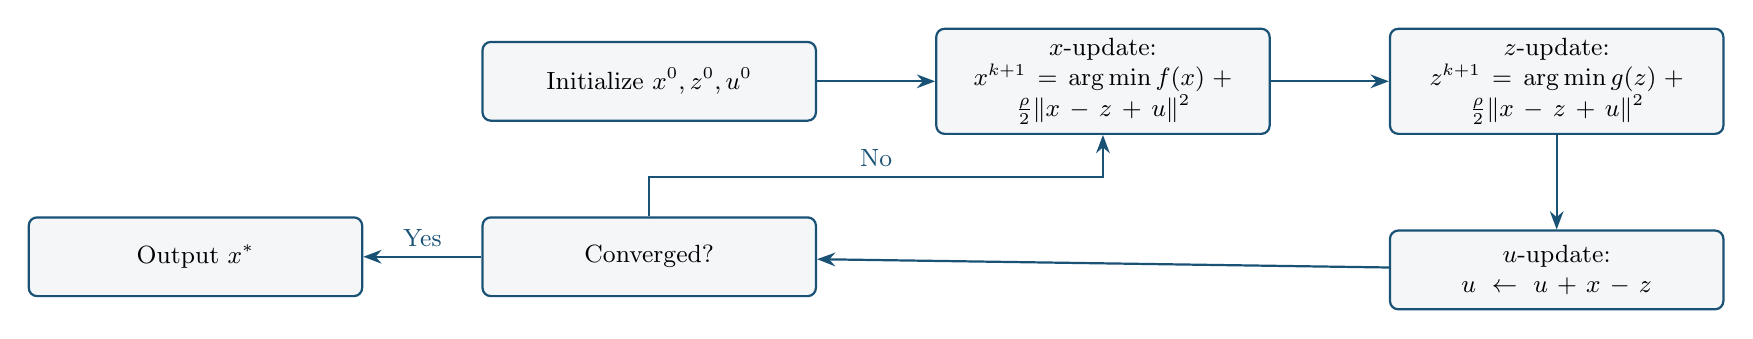
\begin{tikzpicture}[
  node distance=1.2cm and 1.5cm,
  block/.style={rectangle, draw=accent, thick, fill=accent!5,
    text width=4cm, align=center, rounded corners=3pt,
    minimum height=1cm, font=\small},
  arr/.style={-Stealth, thick, accent},
]
\node[block] (init) {Initialize $x^0, z^0, u^0$};
\node[block, right=of init] (xupd) {$x$-update:\\$x^{k+1} = \arg\min f(x) + \frac{\rho}{2}\|x - z + u\|^2$};
\node[block, right=of xupd] (zupd) {$z$-update:\\$z^{k+1} = \arg\min g(z) + \frac{\rho}{2}\|x - z + u\|^2$};
\node[block, below=of zupd] (uupd) {$u$-update:\\$u \gets u + x - z$};
\node[block, below=of init] (check) {Converged?};
\node[block, left=of check] (output) {Output $x^*$};

\draw[arr] (init) -- (xupd);
\draw[arr] (xupd) -- (zupd);
\draw[arr] (zupd) -- (uupd);
\draw[arr] (uupd) -- (check);
\draw[arr] (check) -- node[above]{\small Yes} (output);
\draw[arr] (check.north) -- ++(0,0.5) -| node[pos=0.25,above]{\small No} (xupd.south);
\end{tikzpicture}
\caption{ADMM iteration flowchart: alternating $x$-update, $z$-update,
and dual $u$-update, with convergence check.}
\label{fig:admm_flow}
\end{figure}

% ---- Figure 4: Low-rank matrix geometry (TikZ) ----
\begin{figure}[t]
\centering
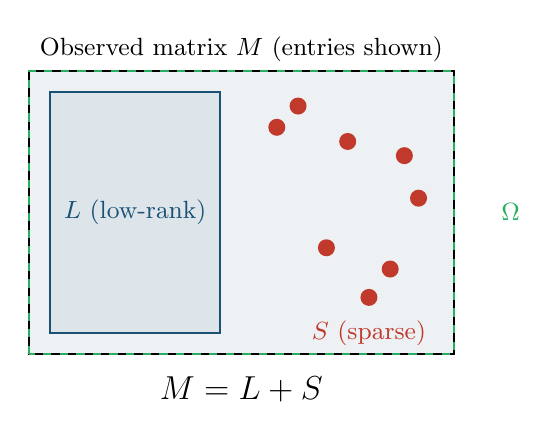
\begin{tikzpicture}[scale=0.9]
% Matrix outline
\draw[thick, fill=accent!8] (0,0) rectangle (6,4);
\node at (3,4.3) {\small Observed matrix $M$ (entries shown)};

% Low-rank part
\draw[thick, accent, fill=accent!15] (0.3,0.3) rectangle (2.7,3.7);
\node[accent] at (1.5,2) {\small $L$ (low-rank)};

% Sparse part
\foreach \x/\y in {3.5/3.2, 4.2/1.5, 5.3/2.8, 4.8/0.8, 3.8/3.5, 5.1/1.2, 4.5/3.0, 5.5/2.2}
  \fill[accent2] (\x,\y) circle (0.12);
\node[accent2] at (4.8,0.3) {\small $S$ (sparse)};

% Equation
\node at (3,-0.5) {\large $M = L + S$};

% Observed mask
\draw[thick, accent3, dashed] (0,0) rectangle (6,4);
\node[accent3] at (6.8,2) {\small $\Omega$};
\end{tikzpicture}
\caption{Robust PCA decomposition: the observed matrix $M$ is the sum of
a low-rank component $L$ and a sparse component $S$.}
\label{fig:rpca}
\end{figure}

% ---- Figure 5: Singular value decay (PGFPlots) ----
\begin{figure}[t]
\centering
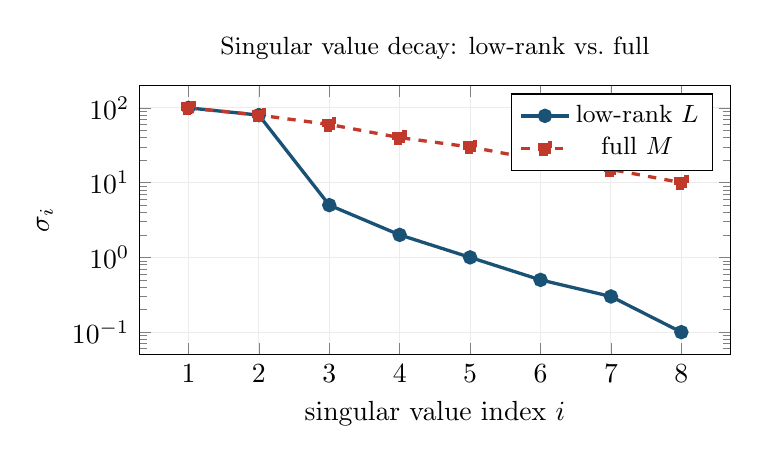
\begin{tikzpicture}
\begin{axis}[
  width=0.75\textwidth, height=5cm,
  xlabel={singular value index $i$}, ylabel={$\sigma_i$},
  ymode=log, grid=major, grid style={gray!15},
  legend pos=north east, legend style={font=\small},
  title={\small Singular value decay: low-rank vs.\ full}
]
\addplot[accent, very thick, mark=*] coordinates {
  (1,100)(2,80)(3,5)(4,2)(5,1)(6,0.5)(7,0.3)(8,0.1)
};
\addlegendentry{low-rank $L$}
\addplot[accent2, very thick, mark=square*, dashed] coordinates {
  (1,100)(2,80)(3,60)(4,40)(5,30)(6,20)(7,15)(8,10)
};
\addlegendentry{full $M$}
\end{axis}
\end{tikzpicture}
\caption{Singular value decay of the low-rank component (rapid drop after
rank $r$) versus the full observed matrix (slow decay due to sparse noise).}
\label{fig:svd_decay}
\end{figure}

% ---- Figure 6: Matrix completion illustration (TikZ) ----
\begin{figure}[t]
\centering
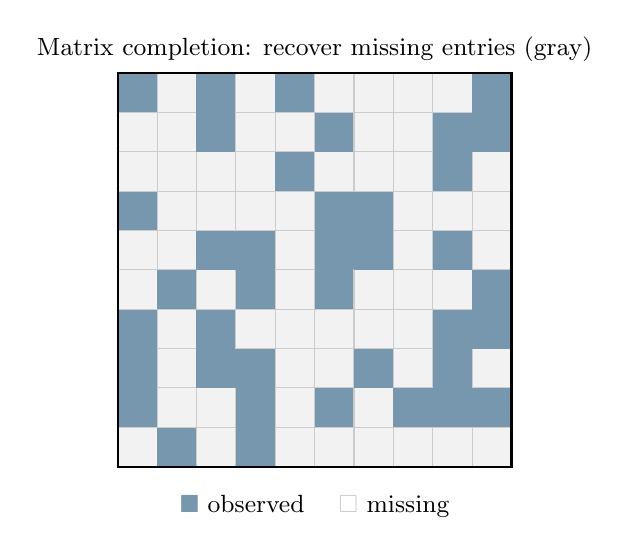
\begin{tikzpicture}[scale=0.5]
\foreach \i in {0,...,9}{
  \foreach \j in {0,...,9}{
    \pgfmathsetmacro{\r}{rand}
    \ifdim\r pt>0.3pt
      \fill[accent!60] (\i,\j) rectangle (\i+1,\j+1);
    \else
      \draw[gray!40, fill=gray!10] (\i,\j) rectangle (\i+1,\j+1);
    \fi
  }
}
\draw[thick] (0,0) rectangle (10,10);
\node at (5,-1) {\small \textcolor{accent!60}{$\blacksquare$} observed \quad
\textcolor{gray!40}{$\square$} missing};
\node at (5,10.6) {\small Matrix completion: recover missing entries (gray)};
\end{tikzpicture}
\caption{Matrix completion: given partial observations (blue), recover the
full low-rank matrix by filling in the missing entries (gray).}
\label{fig:completion}
\end{figure}

% ---- Figure 7: ADMM splitting geometry (TikZ) ----
\begin{figure}[t]
\centering
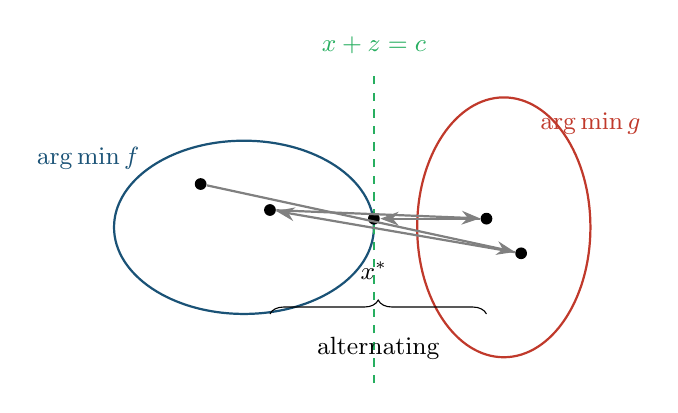
\begin{tikzpicture}[scale=1.1]
% Contour of f
\draw[accent, thick] (0,0) ellipse (1.5 and 1);
\node[accent] at (-1.8,0.8) {\small $\arg\min f$};

% Contour of g
\draw[accent2, thick] (3,0) ellipse (1 and 1.5);
\node[accent2] at (4,1.2) {\small $\arg\min g$};

% Constraint set
\draw[accent3, thick, dashed] (1.5,-1.8) -- (1.5,1.8);
\node[accent3] at (1.5,2.1) {\small $x + z = c$};

% Iterates
\node[fill=black, circle, inner sep=1.5pt] (x0) at (-0.5,0.5) {};
\node[fill=black, circle, inner sep=1.5pt] (z0) at (3.2,-0.3) {};
\node[fill=black, circle, inner sep=1.5pt] (x1) at (0.3,0.2) {};
\node[fill=black, circle, inner sep=1.5pt] (z1) at (2.8,0.1) {};
\node[fill=black, circle, inner sep=1.5pt] (xs) at (1.5,0.1) {};

\draw[-Stealth, gray, thick] (x0) -- (z0);
\draw[-Stealth, gray, thick] (z0) -- (x1);
\draw[-Stealth, gray, thick] (x1) -- (z1);
\draw[-Stealth, gray, thick] (z1) -- (xs);

\node at (1.5,-0.5) {\small $x^*$};

\draw[decorate, decoration={brace, amplitude=5pt}] (0.3,-1) -- (2.8,-1);
\node at (1.55,-1.4) {\small alternating};
\end{tikzpicture}
\caption{ADMM splitting geometry: the algorithm alternates between minimizing
$f$ (left) and $g$ (right), projected onto the constraint $x + z = c$.}
\label{fig:admm_geom}
\end{figure}

% =====================================================================
\section{BibTeX bibliography}
% =====================================================================

This section demonstrates BibTeX integration. The references below are
cited in the text: ADMM was popularized by Boyd et al.~\cite{boyd2011distributed},
robust PCA by Cand\`es et al.~\cite{candes2011robust}, and matrix completion
by Cai et al.~\cite{cai2010singular}.

\bibliography{src/refs}

\end{document}
